\chapter{Technical implementation} \label{technical implementation}

This chapter explains the implementation of our TypeScript application and the Google Cloud infrastructure.
To fulfil the specification for our POC project, we will build a RESTful API with two resources: appointments and practitioners.
The application does not provide all of the CRUD operations (Create, Read, Update and Delete).
Only creating new resources and reading existing ones is supported.
The functionality for updating or deleting resources has not been implemented.
This is done for simplicity, as it is not needed for the scope of the analysis of this thesis.
The program code of a fully implemented application is listed in Appendix \ref{application-code} and infrastructure code in Appendix \ref{infrastructure-code}.

\section{Implementing a minimal application}

In this section, we will build an application matching the specification, except there will be no encryption just yet.
Implementing the encryption is done in the next section.

\subsection{Implementing the TypeScript application}

For the POC project, our application only serves four REST endpoints:
\begin{itemize}
    \item
    \texttt{POST /appointments/} – create a new appointment
    \item
    \texttt{GET /appointments/} – read all the appointments
    \item
    \texttt{POST /practitioners/} – create a new practitioner
    \item
    \texttt{GET /practitioners/} – read all the practitioners
\end{itemize}
The file tree of the application providing these four endpoints is visualized in Figure \ref{fig:filetree}.

\begin{figure}[!htb]
\centering
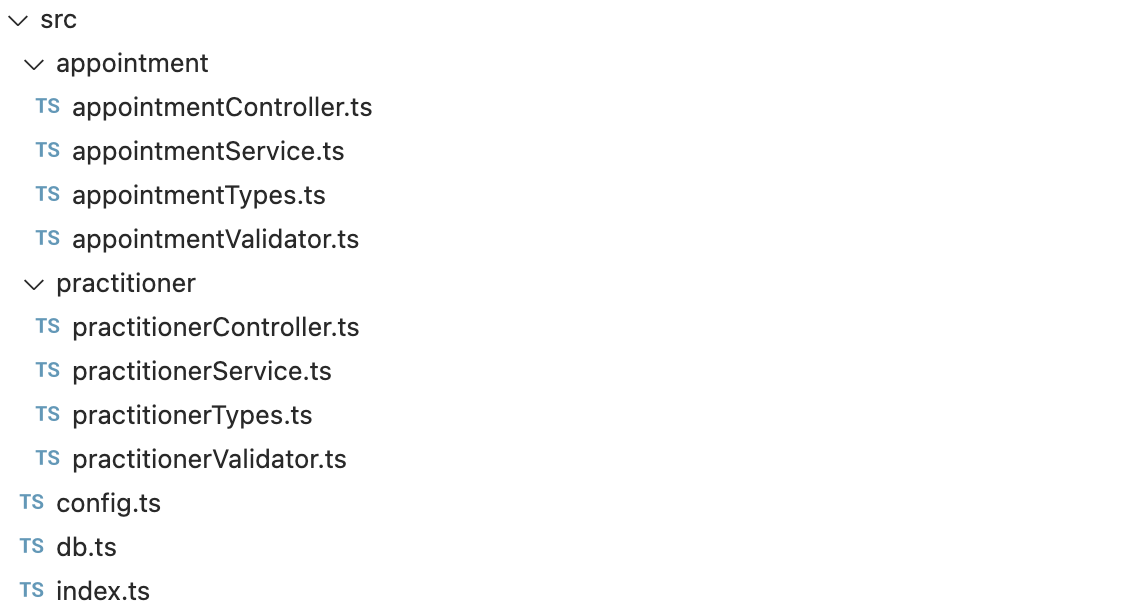
\includegraphics[scale=0.7]{filetree}
\caption{The file tree of a fully functional application}
\label{fig:filetree}
\end{figure}

The role of each file in the application can be understood via a simple request example.
For example, the following is the processing flow of a \texttt{POST /practitioners/} request:
\begin{enumerate}
    \item
    \texttt{index.ts} –
    This is where the Express-application is initialized, along with the middleware.
    From here, the request is routed to the correct controller.
    \item
    \texttt{practitionerController.ts} –
    Handles the routing for the endpoints at\\ \texttt{/appointments/}.
    First, the \texttt{validatePractitioner}-function is called, to validate the body of the request.
    Second, the \texttt{insertPractitioner}-function is called to save the new practitioner.
    \item
    \texttt{practitionerValidator.ts} –
    Validates the body of the request is an object, and it includes the required fields.
    \item
    \texttt{practitionerService.ts} –
    Executes an SQL query and inserts a new row into the database table \texttt{Practitioner}.
\end{enumerate}
A request to the \texttt{POST /appointments/} is handled very similarly, except that there is a relation between the appointment: the practitioner it is being booked for.
So, in addition to the flow explained above, the application checks that the practitioner exists.

A request to either of the \texttt{GET} endpoints does no validation for the request, as there is no body to validate.
It only queries all the rows from the database for the specified resource.

In addition to the files used to handle the request, there are two files not explained yet: \texttt{config.ts} and \texttt{db.ts}.
The former one handles the environment variable configuration in a type safe way: by throwing if the environment variable does not exist.
The latter initializes the database connection.

\subsection{Implementing the Google Cloud infrastructure}

The infrastructure for our POC project is built on the Google Cloud Platform.
It is managed by the Terraform infrastructure-as-code language.
The fully functional infrastructure is visualized in Figure \ref{fig:filetree-infra}.

% My module structure is bad. A quote from Terraform's docs:
% "We do not recommend writing modules that are just thin wrappers around single other resource types. If you have trouble finding a name for your module that isn't the same as the main resource type inside it, that may be a sign that your module is not creating any new abstraction and so the module is adding unnecessary complexity. Just use the resource type directly in the calling module instead."

The role of each notable file and module is as follows:
\begin{itemize}
    \item
    \texttt{gcp\_init.tf} –
    Declare the required version of Terraform and the providers needed.
    Initialize the Google Cloud Platform's provider with the correct project, region and zone.
    \item
    \texttt{main.tf} –
    The constants such as database configuration are declared here.
    All of the modules are are loaded and used here.
    \item
    \texttt{modules/artifact-registry} –
    Creates a private Docker repository for storing the Docker images for our server application.
    \item
    \texttt{modules/cloud-run} –
    Creates and configures a Cloud Run service to run our containerized server application. 
    \item
    \texttt{modules/cloud-sql}
    Creates a database instance with Cloud SQL.
    Creates a database and runs the \texttt{init.sql} script to initialize the tables.
    Adds a database user to the database.
\end{itemize}

\begin{figure}[h!]
\centering
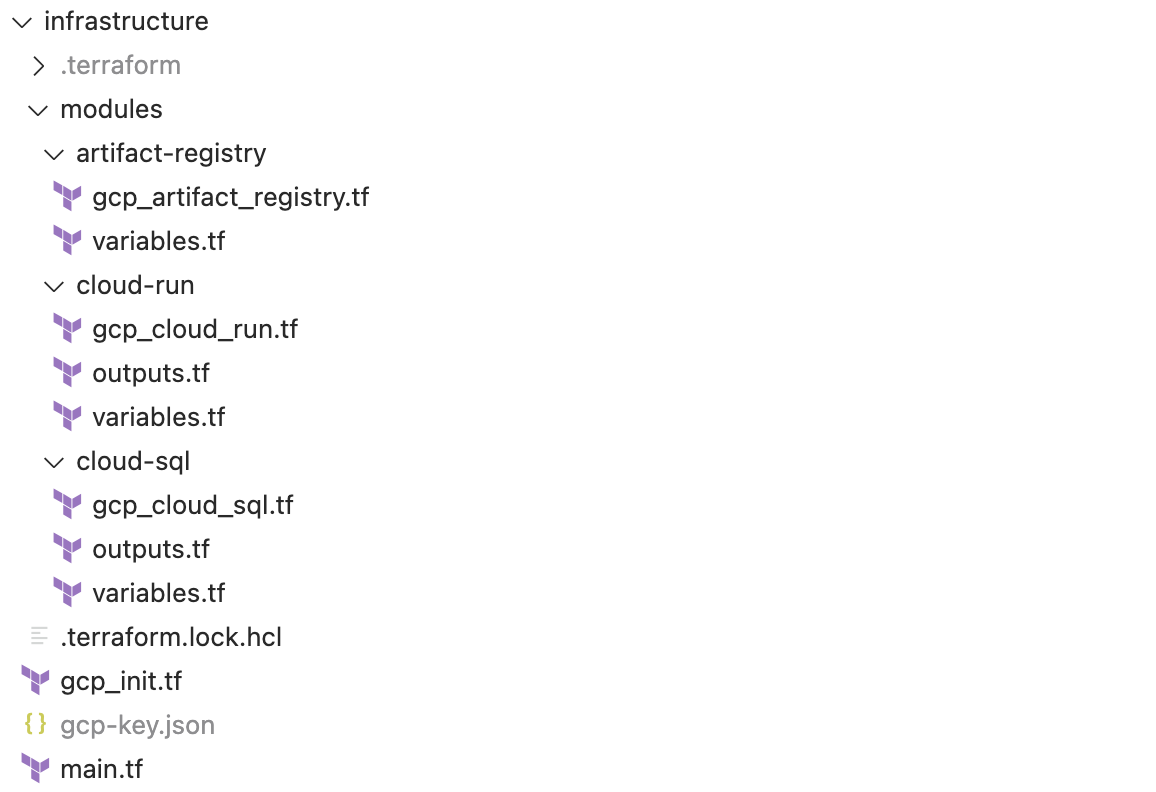
\includegraphics[scale=0.7]{filetree-infra}
\caption{The file tree of a fully functional infrastructure}
\label{fig:filetree-infra}
\end{figure}

Obviously, the implemented POC has numerous limitations.
This is the minimum amount of infrastructure needed to run the application without any encryption for the data.
The secrets are also not handled with a proper solution, as they are plaintext in the infrastructure code.
The routing is not handled to a custom domain either.
However, the application is now accessible to anyone on the internet and this counts as a minimum viable product (MVP) for the POC project specification, albeit without any security measures yet.

\section{Implementing encryption for the application}

In this section, the application and infrastructure built in the section before are improved by adding proper security measures.
We will add envelope encryption to the application and the infrastructure required by it.
The secret environment variables are also moved into GCP's Secret Manager for added security.

\subsection{Implementing envelope encryption in the TypeScript application}

Our encryption-specific code is placed inside \texttt{encryption.ts} file.
First, the application decrypts the key encryption key.
This is done via Google's own \\\texttt{@google-cloud/kms} npm-package. An example implementation is shown in Listing \ref{alg:decrypt-kek}.

\begin{algorithm}[htb]
\begin{minted}{typescript}
const kms = new KeyManagementServiceClient();
const ciphertextBuffer = Buffer.from(KEY_ENCRYPTION_KEY, "base64");
const keyName =
  kms.cryptoKeyPath("dippapoc", "global", KMS_KEYRING, KMS_KEY);
const [decryptResponse] = await kms.decrypt({
  name: keyName,
  ciphertext: ciphertextBuffer,
});
const { plaintext } = decryptResponse;
const keyEncryptionKey = Buffer.from(plaintext);
\end{minted}
\caption{An example implementation for decrypting the key encryption key with Cloud Key Management.}
\label{alg:decrypt-kek}
\end{algorithm}

Inside the \texttt{encrypt.ts} file, we also declare functions for generating, encrypting and decrypting pseudorandom data encryption keys, as well as functions for encrypting and decrypting data with any key provided.
The DEKs are generated using Node.js' built-in crypto-module's pseudorandom data generation via the \texttt{randomBytes}-function.
An example implementation for generating a key is shown in Listing \ref{alg:generate-datakey}.

\begin{algorithm}[htb]
\begin{minted}{typescript}
const generateDataKey = (): Buffer => {
  return crypto.randomBytes(32);
};
export { generateDataKey };
\end{minted}
\caption{An example implementation for generating a pseudorandom data encryption key.}
\label{alg:generate-datakey}
\end{algorithm}

For encrypting and decrypting data we will declare functions in the same file.
Encryption is done with the strong AES-256-CBC algorithm supported by the crypto-module.
Encrypting data is done using crypto-module's \texttt{createCipheriv}-function.
Decrypting data is done similary via the \texttt{createDecipheriv}-function.
An example implementation for implementing encryption and decryption is shown in Listing \ref{alg:encrypt-decrypt}.

\begin{breakablealgorithm}
\caption{An example implementation for AES-256-CBC encryption and decryption.}
\begin{minted}{typescript}
// previous code omitted.
const algorithm = "aes-256-cbc";
const initVector = Buffer.from(CRYPTO_INIT_VECTOR, "hex");
const encrypt = (key: Buffer, plaintext: string) => {
  const cipher = crypto.createCipheriv(algorithm, key, initVector);
  let ciphertext = cipher.update(plaintext, "utf-8", "base64");
  ciphertext +=  cipher.final("base64");
  return ciphertext;
};
const decrypt = (key: Buffer, ciphertext: string) => {
  const decipher =
    crypto.createDecipheriv(algorithm, key, initVector);
  let plaintext = decipher.update(ciphertext, "base64", "utf-8");
  plaintext += decipher.final("utf-8");
  return plaintext;
};
export { /* ... */ encrypt, decrypt };
\end{minted}
\label{alg:encrypt-decrypt}
\end{breakablealgorithm}

The \texttt{encrypt} and \texttt{decrypt} functions created above can be used as-is for encrypting and decrypting the DEKs.
We just need to pass the KEK as the parameter for key.
An example is shown in Listing \ref{alg:encrypt-dek}.

\begin{breakablealgorithm}
\caption{An example implementation for encrypting and decrypting data encryption keys.}
\begin{minted}{typescript}
// previous code omitted.
const encryptDataKey = (dataKey: Buffer): string => {
  const dataKeyString = dataKey.toString("hex");
  return encrypt(keyEncryptionKey, dataKeyString);
};
const decryptDataKey = (dataKey: string): Buffer => {
  const dataKeyString = decrypt(keyEncryptionKey, dataKey);
  return Buffer.from(dataKeyString, "hex");
};
export { /* ... */ encryptDataKey, decryptDataKey };
\end{minted}
\label{alg:encrypt-dek}
\end{breakablealgorithm}

Using the functions declared in the \texttt{encryption.ts}-file, it is possible to encrypt and decrypt any of our data objects and data encryption keys.
As an example for how the functions are used, Listing \ref{alg:encrypt-appointment} implements encryption and decryption for a practitioner-object.
The encryption is done very similarly for an appointment.

\begin{breakablealgorithm}
\caption{An example implementation for encrypting and decrypting a practitioner-object.}
\begin{minted}{typescript}
const encryptPractitioner = (
  practitioner: Practitioner
): EncryptedPractitioner => {
  const key = generateDataKey();
  // Encrypt personal data with the data key
  const firstnames = encrypt(key, practitioner.firstnames);
  const lastname = encrypt(key, practitioner.lastname);
  const education = encrypt(key, practitioner.education);
  // Wrap the data key with the key encryption key
  const data_key = encryptDataKey(key);
  return { firstnames, lastname, education, data_key };
};

const decryptPractitioner = (
  practitioner: EncryptedPractitioner
): Practitioner => {
  const { data_key, id } = practitioner;
  // Decrypt the data key with the key encryption key
  const key = decryptDataKey(data_key);
  // Use the data key to decrypt rest of the fields
  const firstnames = decrypt(key, practitioner.firstnames);
  const lastname = decrypt(key, practitioner.lastname);
  const education = decrypt(key, practitioner.education);
  return { firstnames, lastname, education, id };
};
\end{minted}
\label{alg:encrypt-appointment}
\end{breakablealgorithm}

% Voi myös miettiä, voiko koko ratkaisua/asetelmaa jotenkin esittää myös kuvallisesti
% -SR

\subsection{Implementing infrastructure for envelope encryption}

The application we now have requires new infrastructure to support envelope encryption: Google Cloud Key Management.
On top of adding a KMS key, we will move our secret environment variables such as database configuration and cryptographic secrets into GCP's Secret Manager.

To add Cloud Key Management to the POC application, we need three new resources managed by Terraform:
\begin{itemize}
    \item A KMS keyring to store cryptographic keys
    \item A KMS key to be used for cryptographic operations
    \item A KMS IAM member to update the IAM policy to allow Cloud Run to access it
\end{itemize}
An example implementation is shown in Listing \ref{alg:kms}.

\begin{breakablealgorithm}
\caption{An example implementation for adding Cloud Key Management infrastructure.}
\begin{minted}{terraform}
resource "google_kms_key_ring" "keyring" {
  name     = "dippapoc-keyring"
  location = "global"
}
resource "google_kms_crypto_key" "key" {
  name            = "dippapoc-key"
  key_ring        = google_kms_key_ring.keyring.id
  rotation_period = "2592000s" # 30 days
}

data "google_project" "project" {}
resource "google_kms_crypto_key_iam_member" "kms_compute" {
  crypto_key_id = google_kms_crypto_key.key.id
  role      = "roles/cloudkms.cryptoKeyDecrypter"
  member    = <<EOF
serviceAccount:${
  data.google_project.project.number
}-compute@developer.gserviceaccount.com
EOF
}
\end{minted}
\label{alg:kms}
\end{breakablealgorithm}

Adding the infrastructure for Secret Manager and the secrets themselves is handled by Terraform.
For a single secret that is accessible by Cloud Run, we need three new resources:
\begin{itemize}
    \item A Secret Manager Secret for a logical place to store a single secret
    \item A Secret Manager Secret version which holds the value of the secret itself
    \item A Secret Manager Secret IAM policy to allow Cloud Run to access the secret
\end{itemize}
For ease of use, these resources are bundled into a reusable module, which is called \texttt{./modules/secret} in the example.
Referencing the Secret Manager secrets as Cloud Run environment variables is not very different from referencing the values themselves.
To reference a Secret Manager secret with Terraform in a Cloud Run service config, a \texttt{value\_from} block is used.
An example of this is shown in Listing \ref{alg:secret-manager}.

\begin{breakablealgorithm}
\caption{An example implementation for referencing a Secret Manager secret in a Cloud Run service.}
\begin{minted}{terraform}
resource "google_cloud_run_service" "run_service" {
  name     = var.name
  location = "europe-north1"

  template {
    spec {
      containers {
        image = var.docker_image
        
        env {
          name  = "PGUSER"
          value = var.pguser # the value itself
        }
        env {
          name = "PGPASSWORD"
          value_from {
            secret_key_ref {
              name = var.secret_id_pgpassword # id of a secret
              key  = "latest"
            }
          }
        }
      }
    }
  }
}
\end{minted}
\label{alg:secret-manager}
\end{breakablealgorithm}
